\documentclass[10pt,twocolumn]{article}

\usepackage[utf8]{inputenc}
\usepackage{graphicx}
\usepackage{amsmath}
\usepackage{booktabs}
\usepackage{hyperref}
\usepackage[margin=1in]{geometry}
\usepackage{float}
\usepackage{algorithm}
\usepackage{algpseudocode}
\usepackage{bbm}
\usepackage{subcaption}

% Title information
\title{Lung Cancer Histopathological Classification: \\CNN vs ScatNet Approaches}
\author{Lorenzo Mioso}
\date{April 2025}

\begin{document}

\maketitle

\begin{abstract}
This report compares Convolutional Neural Networks (CNNs) and Scattering Networks (ScatNets) for lung cancer histopathological image classification. Evaluating both models on adenocarcinoma and benign tissue samples, I found that CNNs achieve superior performance (99.26\% accuracy vs ScatNet's 92.99\%), despite ScatNet's theoretical advantages of translation and rotation invariance. Grayscale features proved sufficient for accurate classification, indicating tissue morphology rather than staining drives model decisions. Analysis through guided backpropagation revealed CNNs produce more interpretable and pathologically relevant attribution maps compared to ScatNet's diffuse visualizations.
\end{abstract}

\section{Introduction}
Automated classification of histopathological images plays a crucial role in computer-aided diagnosis systems for cancer detection. This study compares two fundamentally different approaches for classifying lung tissue samples into adenocarcinoma (malignant) and benign categories: Convolutional Neural Networks (CNNs) with learned filters and Scattering Networks (ScatNets) with predefined wavelet filters.

While CNNs have demonstrated remarkable success in image classification tasks, their lack of built-in invariance to transformations and black-box nature remain concerns. ScatNets offer mathematical guarantees of invariance to translations and rotations, potentially beneficial for histopathological image analysis where orientation is not diagnostically significant.

This work compares these approaches not only in terms of classification accuracy but also interpretability, using guided backpropagation to visualize features influencing model decisions and provide insights into their reasoning processes.

\section{Dataset and Preprocessing}
\subsection{Dataset Description}
The dataset consists of lung cancer histopathological images categorized into three classes: adenocarcinoma, squamous cell carcinoma, and benign tissue. For this study, I focus on binary classification between adenocarcinoma and benign tissue. The images are high-resolution (768×768 pixels) microscopic views of lung tissue samples.

\begin{figure}[h]
\centering
\begin{subfigure}{0.48\columnwidth}
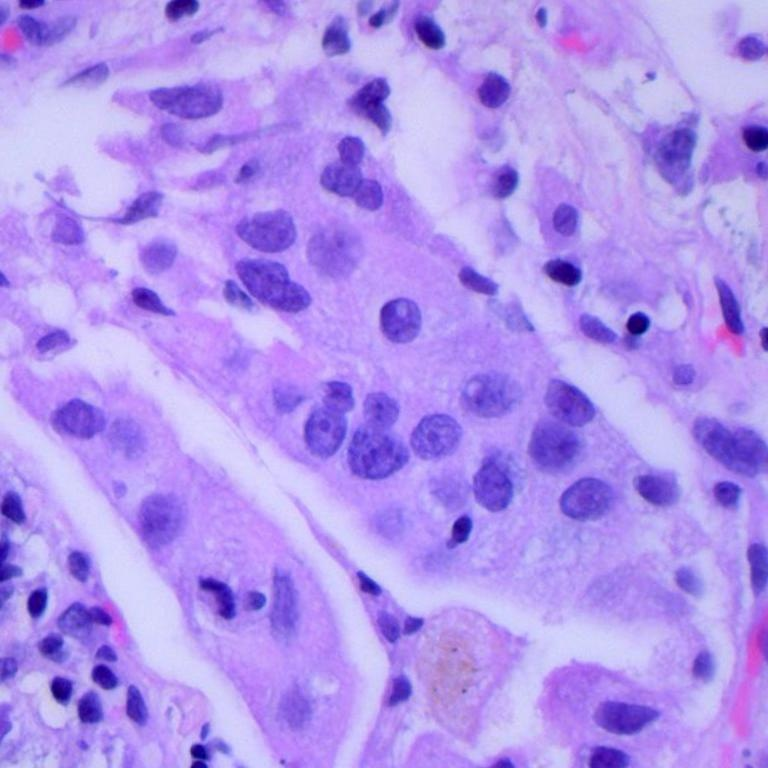
\includegraphics[width=\linewidth]{imgs/adenocarcinoma.jpg}
\caption{Adenocarcinoma sample}
\end{subfigure}
\hfill
\begin{subfigure}{0.48\columnwidth}
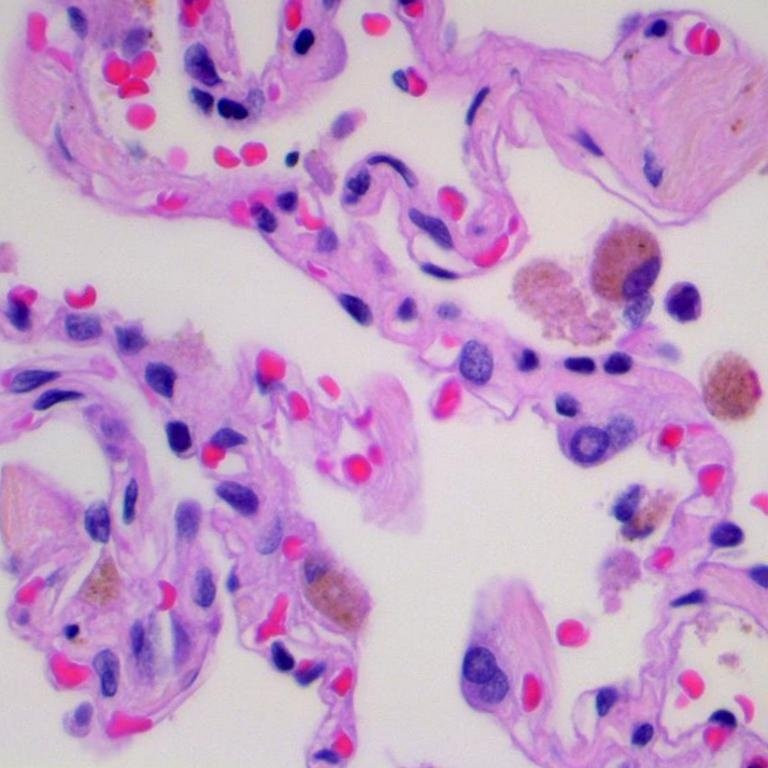
\includegraphics[width=\linewidth]{imgs/benign.jpg}
\caption{Benign tissue sample}
\end{subfigure}
\caption{Representative images from the dataset showing distinct histopathological patterns}
\label{fig:dataset_samples}
\end{figure}

\subsection{Preprocessing Pipeline}
Initial experiments revealed that models achieved near-perfect accuracy by learning color distributions rather than morphological features (Figure \ref{fig:color_distribution}). Since staining variations are not diagnostically relevant, I converted images to grayscale to focus the models on tissue structure.

My preprocessing pipeline included:
\begin{itemize}
    \item Grayscale conversion
    \item Per-fold normalization and standardization
    \item Data augmentation: random rotations, flips, color jittering, cropping, and Gaussian noise
\end{itemize}

Figure \ref{fig:augmentation} demonstrates the effect of augmentation.

\begin{figure}[h]
\centering
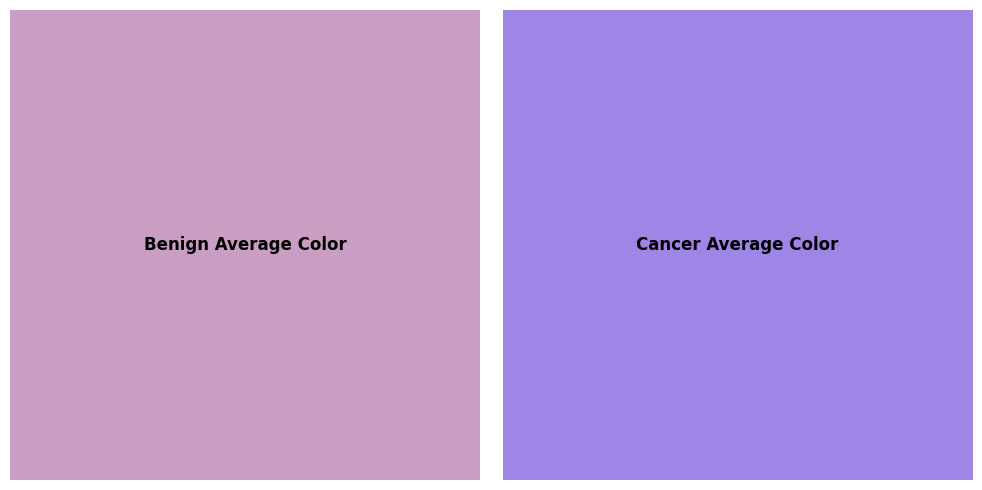
\includegraphics[width=0.8\columnwidth]{imgs/class_avg_colors_horz.png}
\caption{Average color distribution across classes, showing distinct color profiles that could lead to artificial classification cues}
\label{fig:color_distribution}
\end{figure}

\begin{figure}[h]
\centering
\begin{subfigure}{0.48\columnwidth}
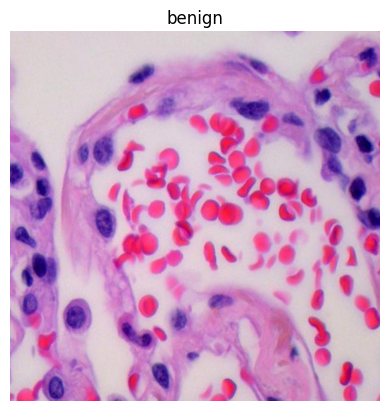
\includegraphics[width=\linewidth]{imgs/normal_image.png}
\caption{Original image}
\end{subfigure}
\hfill
\begin{subfigure}{0.48\columnwidth}
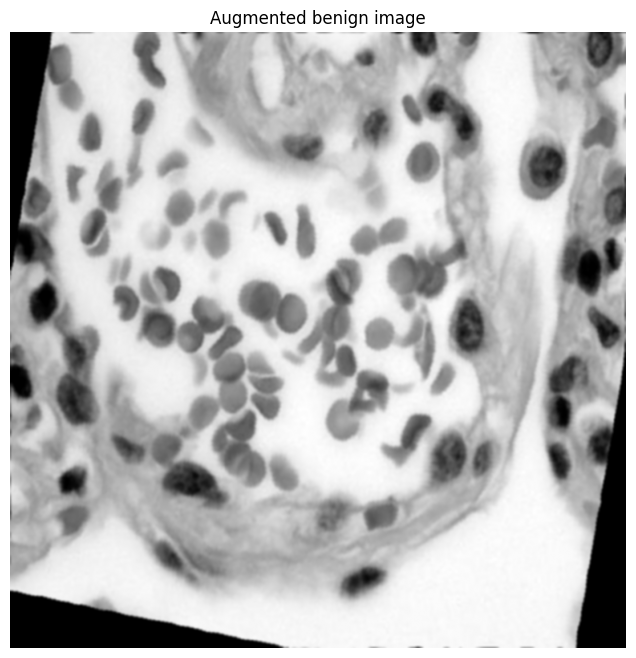
\includegraphics[width=\linewidth]{imgs/augmented_image.png}
\caption{Augmented image}
\end{subfigure}
\caption{Example of data augmentation applied to a histopathological image}
\label{fig:augmentation}
\end{figure}

\section{Model Architectures}
\subsection{CNN Architecture}
I designed an efficient CNN architecture inspired by ResNet but without skip connections. The model consists of three progressive convolutional blocks with increasing filter complexity (16→16→24 filters), as illustrated in Figure \ref{fig:cnn_arch}.

\begin{figure}[h]
\centering
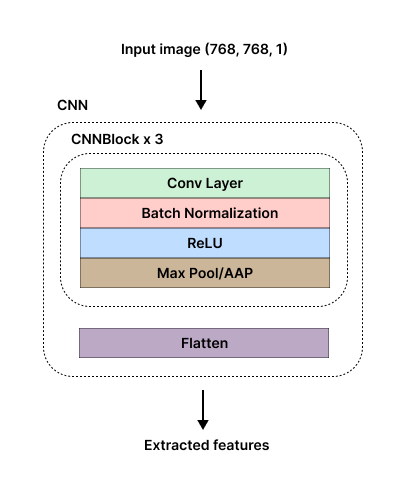
\includegraphics[width=0.9\columnwidth]{imgs/cnn_arch.png}
\caption{CNN architecture with three convolutional blocks followed by a classifier}
\label{fig:cnn_arch}
\end{figure}

Key architectural elements include:
\begin{itemize}
    \item Initial 11×11 convolutional kernel to capture broad tissue patterns
    \item Strategic max pooling for dimensionality reduction
    \item Batch normalization after each convolutional layer
    \item ReLU activations for modeling non-linear relationships
\end{itemize}

\subsection{Scattering Transform}
The scattering transform is a mathematical operation that creates representations of signals invariant to translations and stable to deformations. It operates by cascading wavelet transforms with non-linear modulus operators, followed by local averaging.

The process works in multiple stages:
\begin{itemize}
    \item First-order coefficients capture basic edge and texture information
    \item Second-order coefficients extract more complex patterns resistant to deformation
    \item Low-pass filtering provides translation invariance while preserving spatial information
\end{itemize}

Figure \ref{fig:scat_transform} illustrates the cascaded structure of the scattering transform, where each level provides increasing invariance to geometrical transformations while preserving discriminative information.

\begin{figure}[h]
\centering
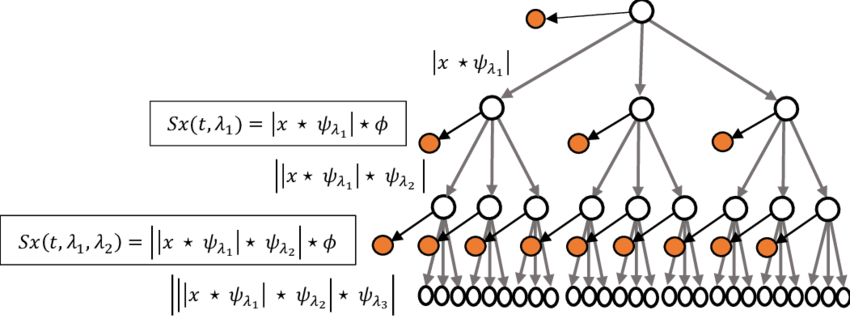
\includegraphics[width=0.9\columnwidth]{imgs/scat_transform.png}
\caption{Diagram of the scattering transform showing wavelet decomposition and feature extraction process}
\label{fig:scat_transform}
\end{figure}

Unlike CNNs, which learn filters from data, the scattering transform uses predefined wavelet filters with mathematical guarantees. This approach offers several advantages for image analysis, including stability to small deformations, preservation of high-frequency information, and reduced sensitivity to rotation and scale changes—qualities potentially beneficial for analyzing biological structures in medical imaging.

\subsection{ScatNet Architecture}
The ScatNet architecture employs wavelet scattering transforms rather than learned filters. My implementation uses:
\begin{itemize}
    \item J=3 scale parameter for wavelet decomposition
    \item L=8 orientations for directional sensitivity
    \item M=2 scattering order to capture higher-order interactions
    \item 4×4 global average pooling to reduce dimensionality
\end{itemize}

The ScatNet processes images through a series of wavelet transformations, producing 3,472 translation, rotation, and scaling invariant features that are then fed to the classifier, as shown in Figure \ref{fig:scatnet_arch}.

\begin{figure}[h]
\centering
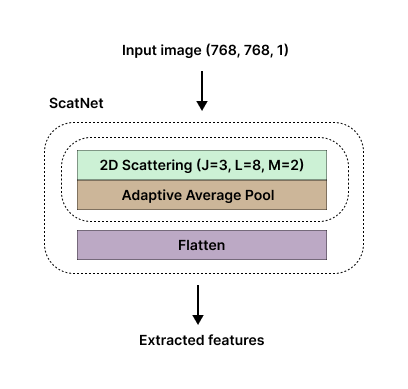
\includegraphics[width=0.9\columnwidth]{imgs/scatnet_arch.png}
\caption{ScatNet architecture with wavelet transforms and classifier}
\label{fig:scatnet_arch}
\end{figure}

\subsection{Feature Classifier}
Both the CNN and ScatNet feature extractors feed into the same classifier architecture:
\begin{itemize}
    \item Single hidden layer with 16 neurons
    \item Batch normalization for training stability
    \item ReLU activation for non-linear patterns
    \item Dropout (0.5) for regularization
    \item Output layer with 2 neurons and softmax activation
\end{itemize}

\begin{figure}[h]
\centering
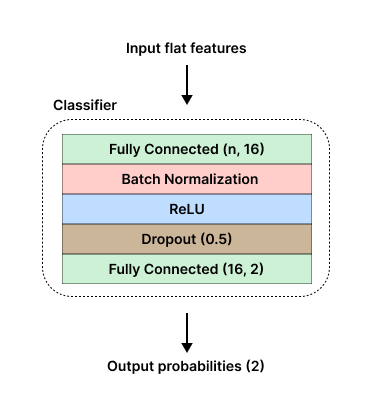
\includegraphics[width=0.8\columnwidth]{imgs/classifier_arch.png}
\caption{Feature classifier architecture used with both CNN and ScatNet}
\label{fig:classifier_arch}
\end{figure}

\section{Training and Evaluation}
\subsection{Training Methodology}
Both models were trained using 10-fold cross-validation with Adam optimizer, but required different learning rate approaches. CNNs benefited from higher learning rates (1e-3 to 5e-3) to develop effective filters capturing subtle tissue patterns, while ScatNet used more conservative rates. The CNN demonstrated rapid convergence (typically within 15 epochs) with minimal overfitting and consistent performance across folds. In contrast, ScatNet required fewer training epochs but showed slower per-epoch convergence and greater cross-fold variance. Early stopping was implemented to prevent overfitting, with model checkpointing to save the best-performing weights.

\section{Results and Analysis}
\subsection{Performance Metrics}
Both models were evaluated using accuracy and F1 score across all 10 folds. Table \ref{tab:performance} summarizes the comparative performance.

\begin{table}[h]
\centering
\caption{Performance comparison between CNN and ScatNet}
\label{tab:performance}
\begin{tabular}{lll}
\toprule
Metric & CNN & ScatNet \\
\midrule
Mean Accuracy & 99.26\% ± 0.72\% & 92.99\% ± 1.59\% \\
Mean F1 Score & 99.27\% ± 0.72\% & 92.83\% ± 1.70\% \\
Best Fold & 99.90\% (Fold 9) & 95.10\% (Fold 6) \\
\bottomrule
\end{tabular}
\end{table}

The CNN significantly outperformed ScatNet by 6.27\% in mean accuracy. Furthermore, the CNN demonstrated more consistent performance across folds, with a standard deviation of 0.72\% compared to ScatNet's 1.59\%.

\subsection{Performance Comparison}
Both models showed strong performance, with CNN significantly outperforming ScatNet:

\begin{itemize}
    \item \textbf{CNN}: Achieved exceptional accuracy (98.00\%-99.90\%) and F1 scores (98.01\%-99.90\%) across all folds, with the best performance in Fold 9 (99.90\% accuracy).
    
    \item \textbf{ScatNet}: Demonstrated good but less consistent performance with accuracy ranging from 89.10\% to 95.10\% and F1 scores from 88.68\% to 95.06\%. The best performing fold was Fold 6 (95.10\%), while Fold 1 performed worst (89.10\%).
\end{itemize}

CNN not only achieved higher peak performance but also showed greater consistency across folds, with a standard deviation of 0.72\% compared to ScatNet's 1.59\%.

\section{Feature Analysis}
\subsection{CNN Filter Analysis}
Visual inspection of the first-layer CNN filters revealed structured patterns relevant to histopathological analysis, as shown in Figure \ref{fig:cnn_filters}.

\begin{figure}[h]
\centering
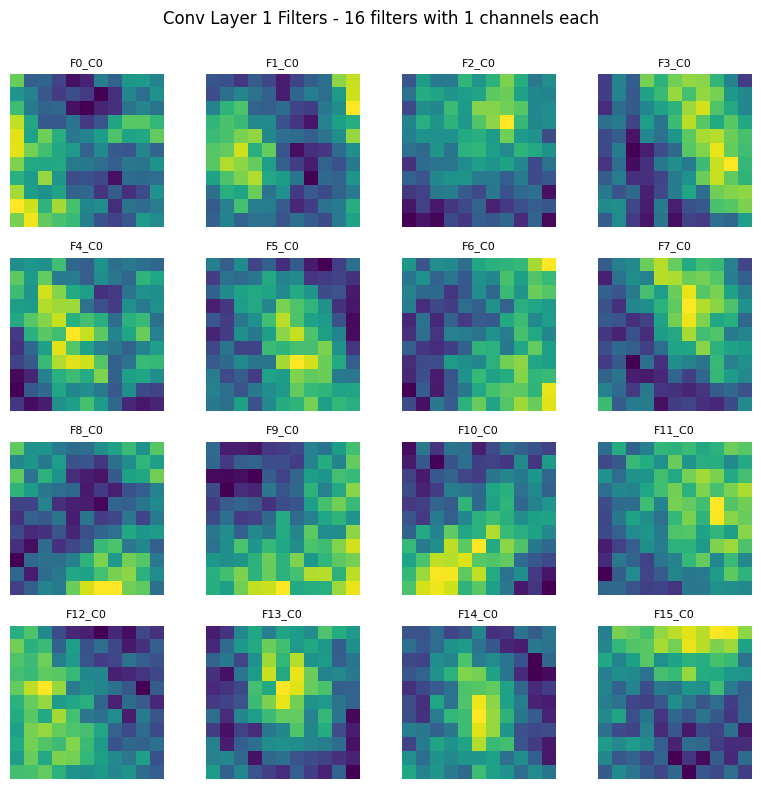
\includegraphics[width=0.8\columnwidth]{imgs/cnn_filters.png}
\caption{Learned filters from the first convolutional layer of the CNN}
\label{fig:cnn_filters}
\end{figure}

The filters exhibited several distinct patterns:
\begin{itemize}
    \item Diagonal and vertical strips for detecting edges and transitions between tissue textures
    \item Circular patterns for identifying cell nuclei and localized features
    \item Two-part filters capturing gradients and contrast changes
\end{itemize}

These patterns align with pathologically relevant features in histological images, such as cell boundaries, nuclei clustering, and tissue organization differences between normal and malignant samples.

\subsection{ScatNet Filter Analysis}
Unlike CNN, ScatNet uses predefined wavelet filters rather than learned ones. Figure \ref{fig:scatnet_filters} shows representative ScatNet filters.

\begin{figure}[h]
\centering
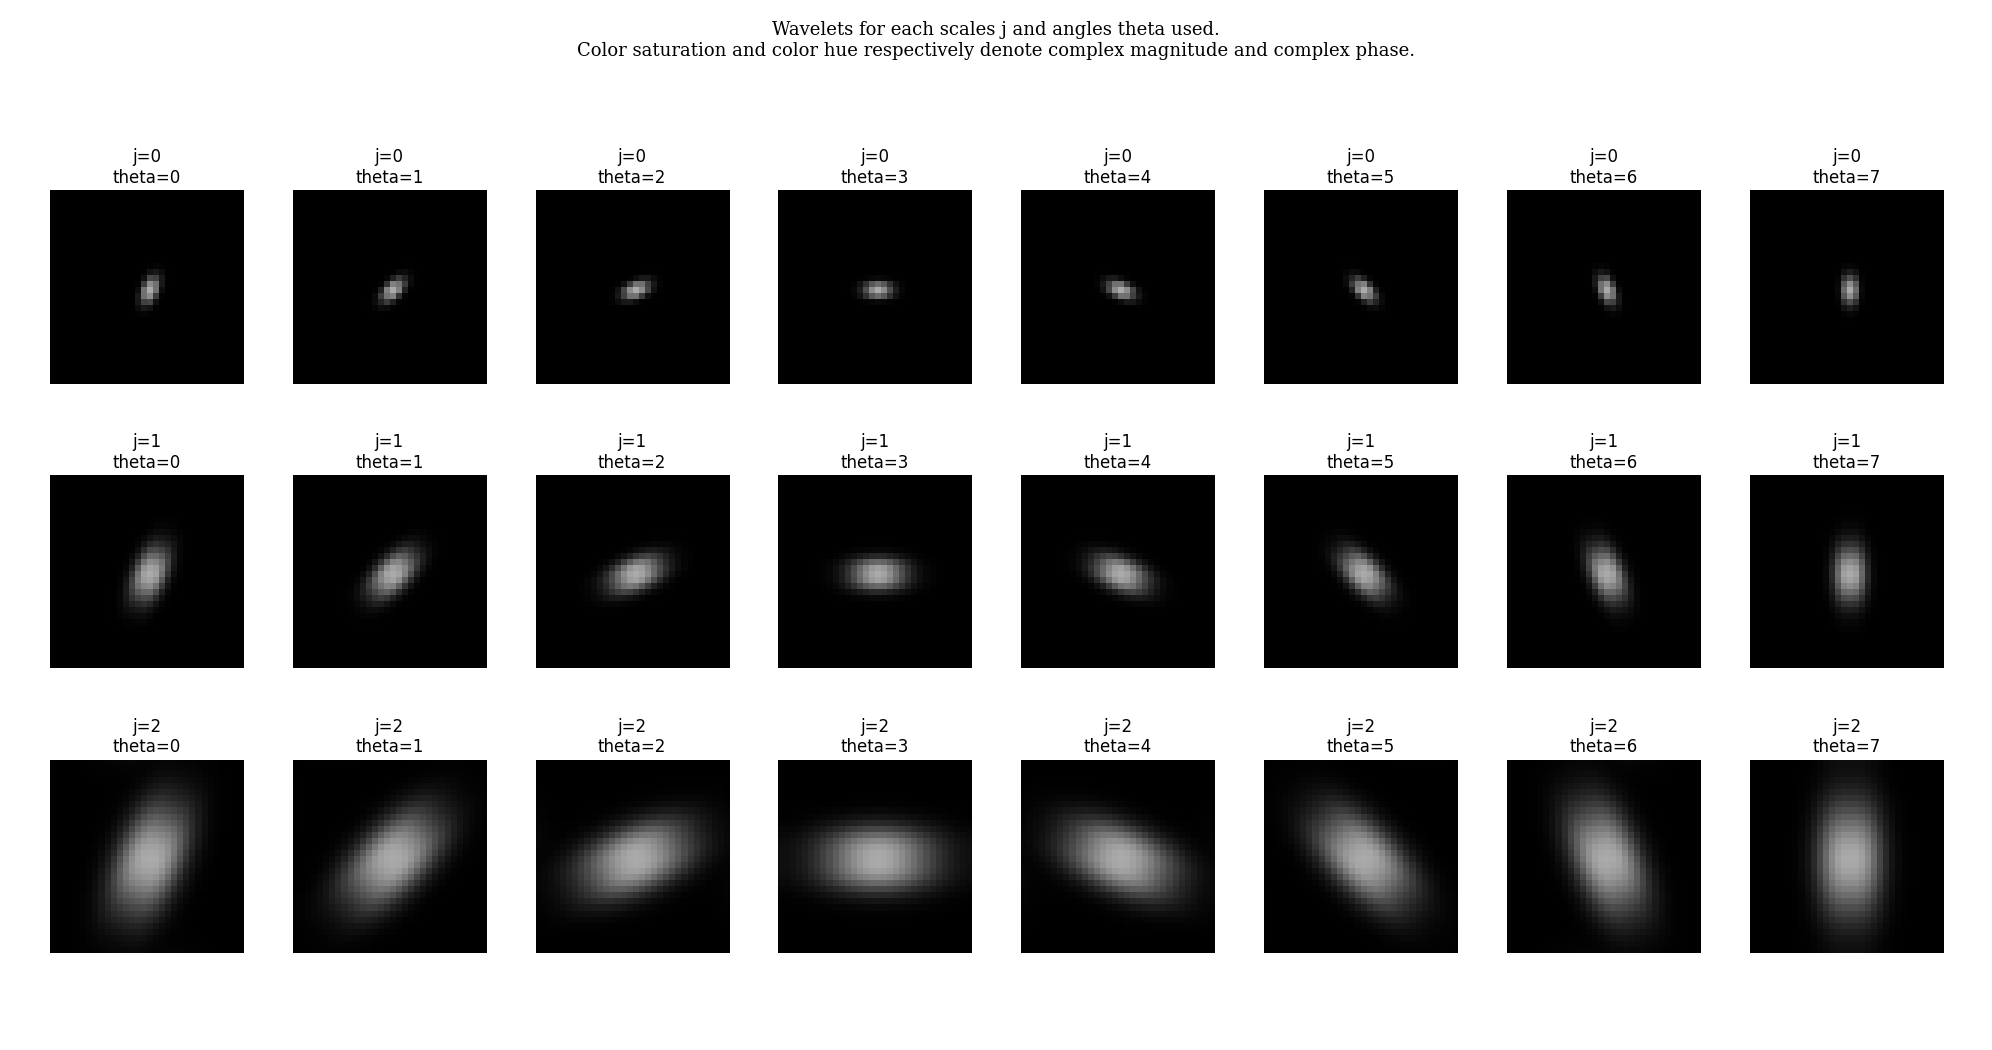
\includegraphics[width=0.7\columnwidth]{imgs/scatnet_filters.png}
\caption{Predefined wavelet filters used in ScatNet}
\label{fig:scatnet_filters}
\end{figure}

While these filters provide theoretical advantages:
\begin{itemize}
    \item Scale and rotation invariance
    \item Mathematical guarantees on stability
    \item No learning required
\end{itemize}

Their fixed nature limits adaptability to the specific characteristics of histopathological images, potentially explaining ScatNet's lower performance despite its solid theoretical foundation.

\section{Guided Backpropagation for Model Interpretation}
\subsection{Methodology}
Guided backpropagation is an enhancement of standard backpropagation that helps visualize which image regions most influence a neural network's classification decision. This technique functions by:

\begin{enumerate}
    \item Starting with a forward pass through the network
    \item Computing gradients of the output with respect to the input image
    \item Modifying the backpropagation of ReLU layers to only allow positive gradients to flow through positive activations
\end{enumerate}

This approach produces clearer, less noisy visualizations by eliminating negative influences that typically create visual noise in standard backpropagation. The result is a saliency map that highlights image regions most strongly activating the target class.

Mathematically, guided backpropagation modifies the gradient flow through ReLU layers as follows:

\begin{equation}
\frac{\partial y}{\partial x} = \frac{\partial y}{\partial f} \cdot \mathbbm{1}_{x > 0} \cdot \mathbbm{1}_{\frac{\partial y}{\partial f} > 0}
\end{equation}

Where $x$ is the input to the ReLU, $f$ is the output, $y$ is the target output, and $\mathbbm{1}$ is the indicator function.

\subsection{CNN Attribution Analysis}
Guided backpropagation revealed distinctive patterns in the CNN's decision-making process, as shown in Figure \ref{fig:cnn_attribution}.

\begin{figure}[h]
\centering
\begin{subfigure}{0.32\columnwidth}
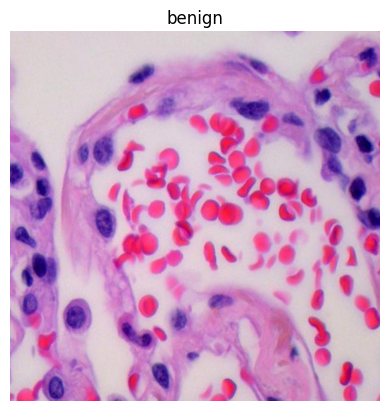
\includegraphics[width=\linewidth]{imgs/normal_image.png}
\caption{Original image}
\end{subfigure}
\hfill
\begin{subfigure}{0.32\columnwidth}
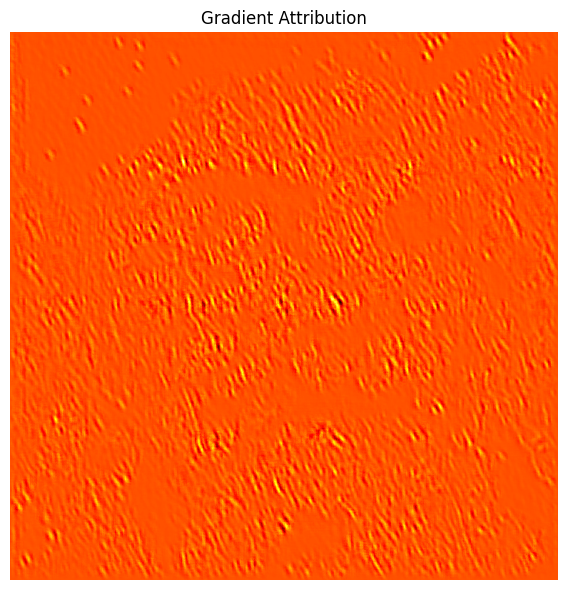
\includegraphics[width=\linewidth]{imgs/cnn_bp.png}
\caption{Standard backprop}
\end{subfigure}
\hfill
\begin{subfigure}{0.32\columnwidth}
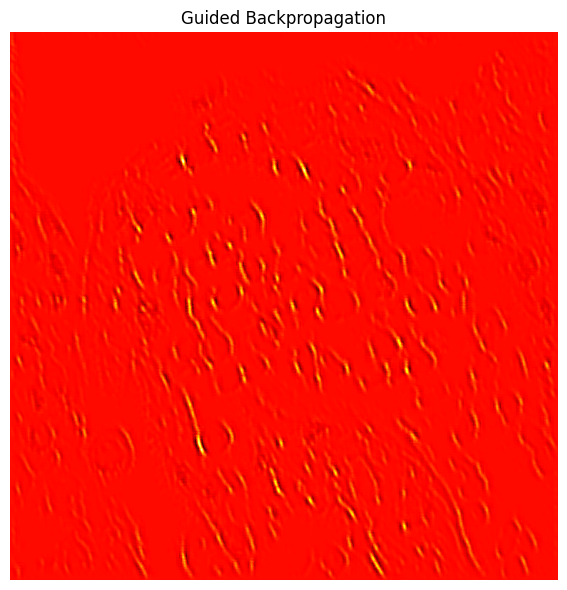
\includegraphics[width=\linewidth]{imgs/cnn_gbp.png}
\caption{Guided backprop}
\end{subfigure}
\caption{CNN attribution analysis comparing standard and guided backpropagation}
\label{fig:cnn_attribution}
\end{figure}

Key observations:
\begin{itemize}
    \item Guided backpropagation significantly reduced noise compared to regular backpropagation
    \item Higher resolution feature attribution with clearer cellular structure patterns
    \item Strong correlation with pathologically relevant regions
    \item Consistent visualization patterns across different implementation methods
\end{itemize}

The guided backpropagation visualizations for CNN highlighted cellular structures and tissue organization patterns that pathologists would typically examine, suggesting that the model focuses on clinically relevant features.

\subsection{ScatNet Attribution Analysis}
ScatNet's attribution maps showed markedly different characteristics, as illustrated in Figure \ref{fig:scatnet_attribution}.

\begin{figure}[h]
\centering
\begin{subfigure}{0.32\columnwidth}
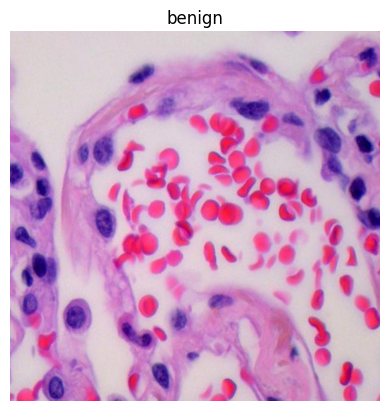
\includegraphics[width=\linewidth]{imgs/normal_image.png}
\caption{Original image}
\end{subfigure}
\hfill
\begin{subfigure}{0.32\columnwidth}
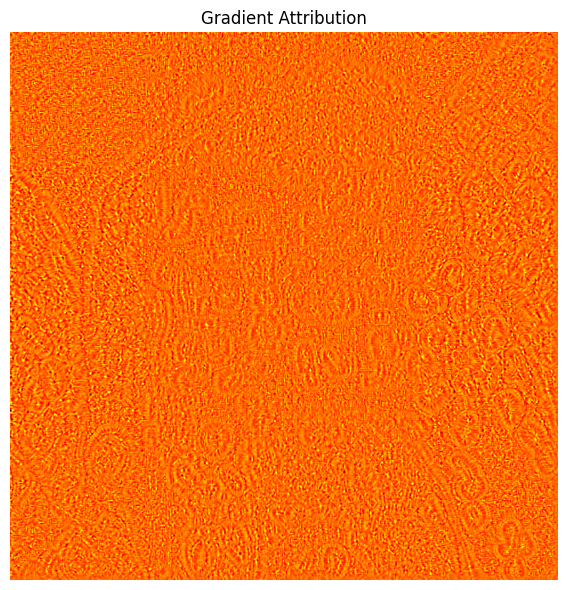
\includegraphics[width=\linewidth]{imgs/scatnet_bp.png}
\caption{Standard backprop}
\end{subfigure}
\hfill
\begin{subfigure}{0.32\columnwidth}
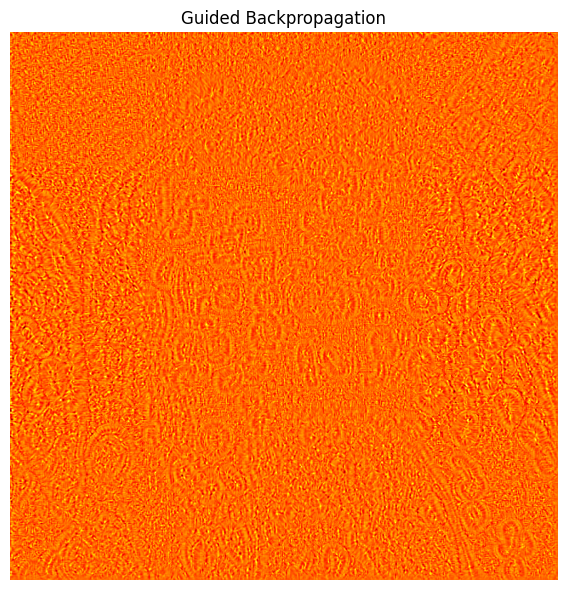
\includegraphics[width=\linewidth]{imgs/scatnet_gbp.png}
\caption{Guided backprop}
\end{subfigure}
\caption{ScatNet attribution analysis comparing standard and guided backpropagation}
\label{fig:scatnet_attribution}
\end{figure}

Notable differences:
\begin{itemize}
    \item Minimal differences between guided and regular backpropagation
    \item Less interpretable, diffuse attribution regions
    \item Weaker correlation with pathologically significant structures
    \item Limited impact of guided backpropagation due to ReLUs only in the classifier layers
\end{itemize}

The limited improvement seen with guided backpropagation in ScatNet can be attributed to its architecture, where non-linearities (ReLU) are only present in the classifier component, not in the feature extraction process. This architectural difference significantly affects how attribution methods perform.

\section{Discussion}
\subsection{Performance Gap Analysis}
The substantial performance gap between CNN and ScatNet (6.27\% mean accuracy difference) can be attributed to several factors:

\begin{itemize}
    \item \textbf{Adaptability}: CNN filters are learned specifically for the histopathology domain, while ScatNet uses fixed mathematical wavelets.
    \item \textbf{Feature specificity}: CNN develops task-specific feature detectors that identify diagnostically relevant patterns in lung tissue.
    \item \textbf{Hierarchical learning}: CNN's multi-layer structure progressively builds more complex feature representations.
    \item \textbf{Over-generalization}: ScatNet's invariance properties, while theoretically advantageous, may discard discriminative information relevant to cancer detection.
\end{itemize}

\subsection{Interpretability Comparison}
From an interpretability perspective:
\begin{itemize}
    \item CNN attribution maps showed stronger correspondence with pathologically relevant structures
    \item ScatNet attribution maps were more diffuse and less aligned with cellular structures
    \item Guided backpropagation significantly enhanced CNN visualizations but had minimal impact on ScatNet visualizations
\end{itemize}

These findings suggest that while ScatNet has theoretical interpretability advantages due to its mathematical foundation, in practice, CNN produces more clinically interpretable explanations.

\subsection{Color vs. Structure}
My experiments confirmed that grayscale images provided sufficient information for accurate classification. This finding has important implications:
\begin{itemize}
    \item Tissue morphology, not staining characteristics, drives model decisions
    \item Models are less likely to be affected by staining variations between laboratories
    \item Potential for application to unstained or differently stained samples
\end{itemize}

\section{Limitations}
Despite the strong results, this study has several limitations that should be acknowledged:

\begin{itemize}
    \item \textbf{Dataset diversity}: The analysis is limited to a single institutional dataset, which may not capture the full spectrum of tissue appearance variations across different laboratories and staining protocols.
    
    \item \textbf{Binary classification focus}: The study addresses only binary classification (adenocarcinoma vs. benign), whereas clinical applications often require multi-class discrimination between different cancer subtypes.
    
    \item \textbf{Fixed architecture comparison}: The comparison evaluates specific implementations of CNN and ScatNet rather than the full range of possible architectures within each approach.
    
    \item \textbf{Limited interpretability methods}: While guided backpropagation provides valuable insights, additional explainability techniques could offer complementary perspectives on model decision processes.
\end{itemize}

\section{Conclusion}
This study compared CNN and ScatNet approaches for lung cancer histopathological image classification, evaluating both performance and interpretability aspects. My findings clearly demonstrate that CNN outperforms ScatNet in this domain despite ScatNet's theoretical advantages.

The superior performance of CNNs can be attributed to their ability to learn domain-specific features directly from the data, adapting to the unique characteristics of histopathological images. The guided backpropagation analysis further revealed that CNN models focus on pathologically relevant regions, providing more interpretable and clinically aligned visualizations than ScatNet.

Based on these findings, I recommend:
\begin{itemize}
    \item \textbf{Clinical implementation}: Deploy CNN-based systems for computer-aided diagnosis in lung histopathology with confidence in their accuracy and interpretability.
    \item \textbf{Model validation}: Conduct multi-center validation studies to verify CNN performance across different laboratory and staining protocols.
    \item \textbf{Feature extraction}: Consider using the identified CNN filters as standardized feature extractors for other histopathology applications.
    \item \textbf{Interpretability tools}: Integrate guided backpropagation visualization into pathologist workflow to enhance model trust and adoption.
\end{itemize}

Future work should explore hybrid approaches combining the adaptability of CNNs with the mathematical guarantees of ScatNets to potentially achieve both high performance and robust interpretability.

\end{document}